\section{Experimental Results}
\label{sec:eval} In this section, we first give some statistics of
our corpus and the extracted causal network, and then evaluate the
quantity and quality of the cue patterns used in the extraction. We
further compare the end-to-end results on COPA task with several
previously published results. We then evaluate our commonsense reasoning
ability on two additional tasks using data from ConceptNet 4 to
further showcase the power of our framework. Finally, we demonstrate
this network's ability to identify causal directions
using annotated corpus of SemEval-2010 task 8, despite being
agnostic about the context of the input word pairs.

The demo of the extracted network, its complete data,
as well as the test sets we use in this section
are available at \url{http://202.120.38.146/causal}.
Further discussion of this demo is included
in \secref{sec:discuss}.
%This section presets our training setting and
%show our results for two tasks.

\subsection{Data Set and Extraction of Causal Network}
\label{sec:causalnet}
\begin{figure*}[th]
\centering
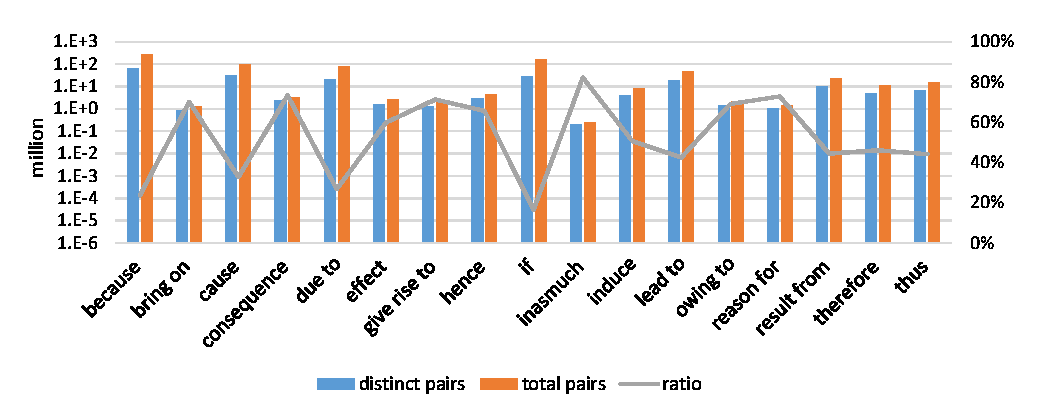
\epsfig{file=pattern1.eps, width=1.6\columnwidth}
%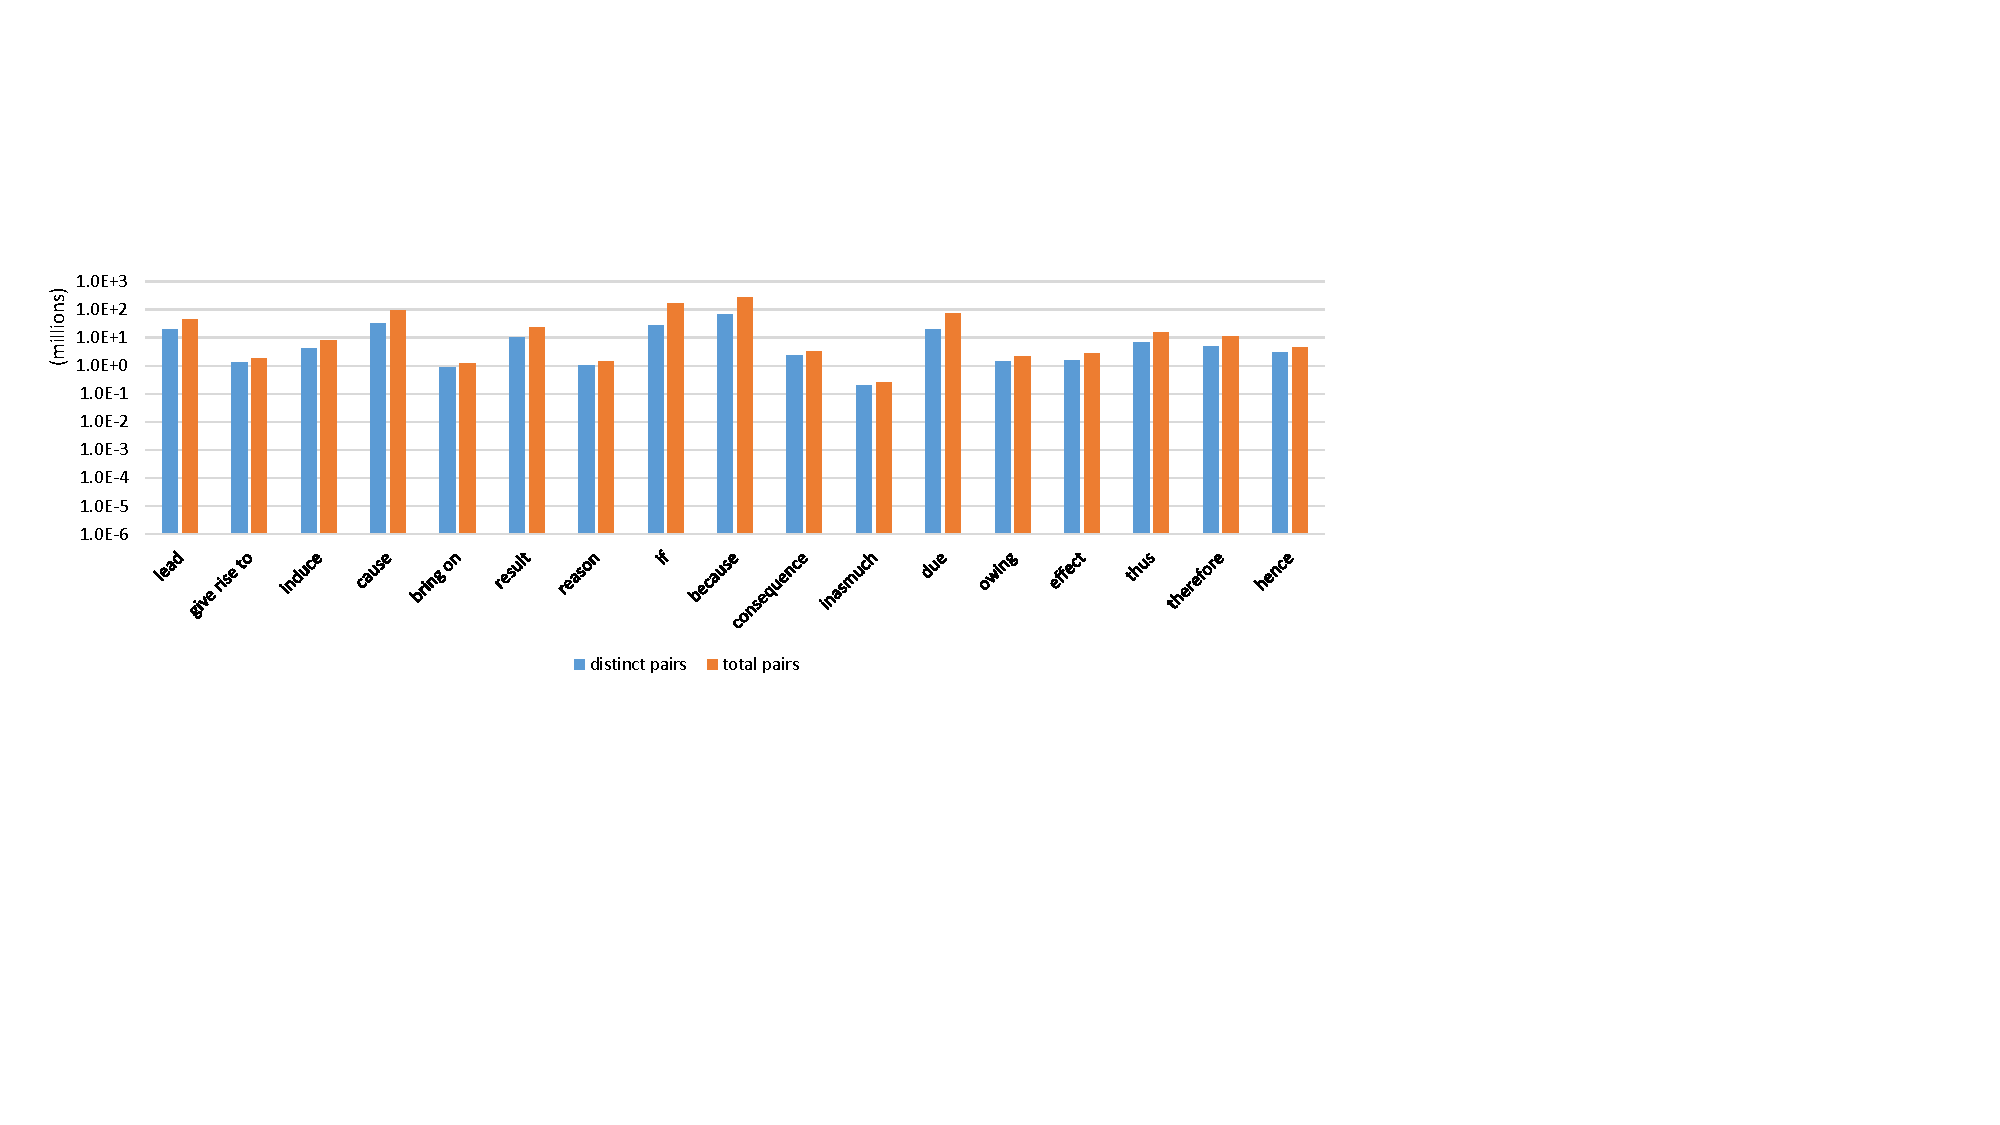
\includegraphics[width=2\columnwidth]{pattern.pdf}
\caption{Number of (distinct) pairs extracted by cues}
\label{fig:pattern1}
\end{figure*}
We extracted our term causality network, which we call ``CausalNet''
for convenience in this section, from a large web text corpus (approximately
10TB), %The snapshot was generated in February, 2013
which contains about 1.6 billion web pages.
We extract 68,217,404 distinct word pairs from this corpus,
which amounts to roughly 8GB. The number of unique lemmatized words
in these pairs is 64,436, covering 41.49\% (64,436/155,287) of the
words in WordNet.

The 53 causal cues we used can be grouped into 17 sets, each
containing cues of the same meaning or lemma form but with different
tenses. Word pair distribution over these sets is shown in Figure
\ref{fig:pattern1}. The blue bars (left) are the number of distinct
pairs and the orange ones (right) show the total number of pairs.
Inter-sentence cues like ``if'' and ``because'' harvested the
largest number of pairs. But more specific patterns such as
``reason'' and ``inasmuch'' find more diverse pairs, since the
number of distinct pairs is relatively large compared to the total
pairs extracted.

\begin{figure*}[th]
\centering
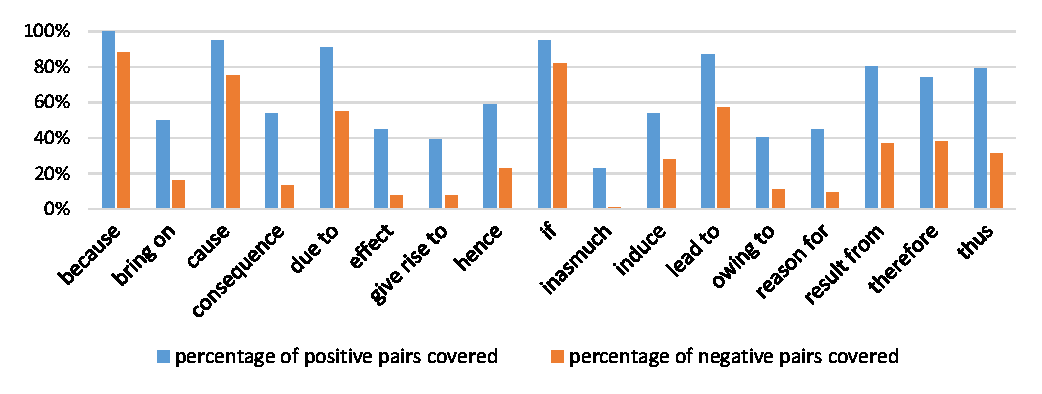
\epsfig{file=pattern3.eps, width=1.6\columnwidth}
%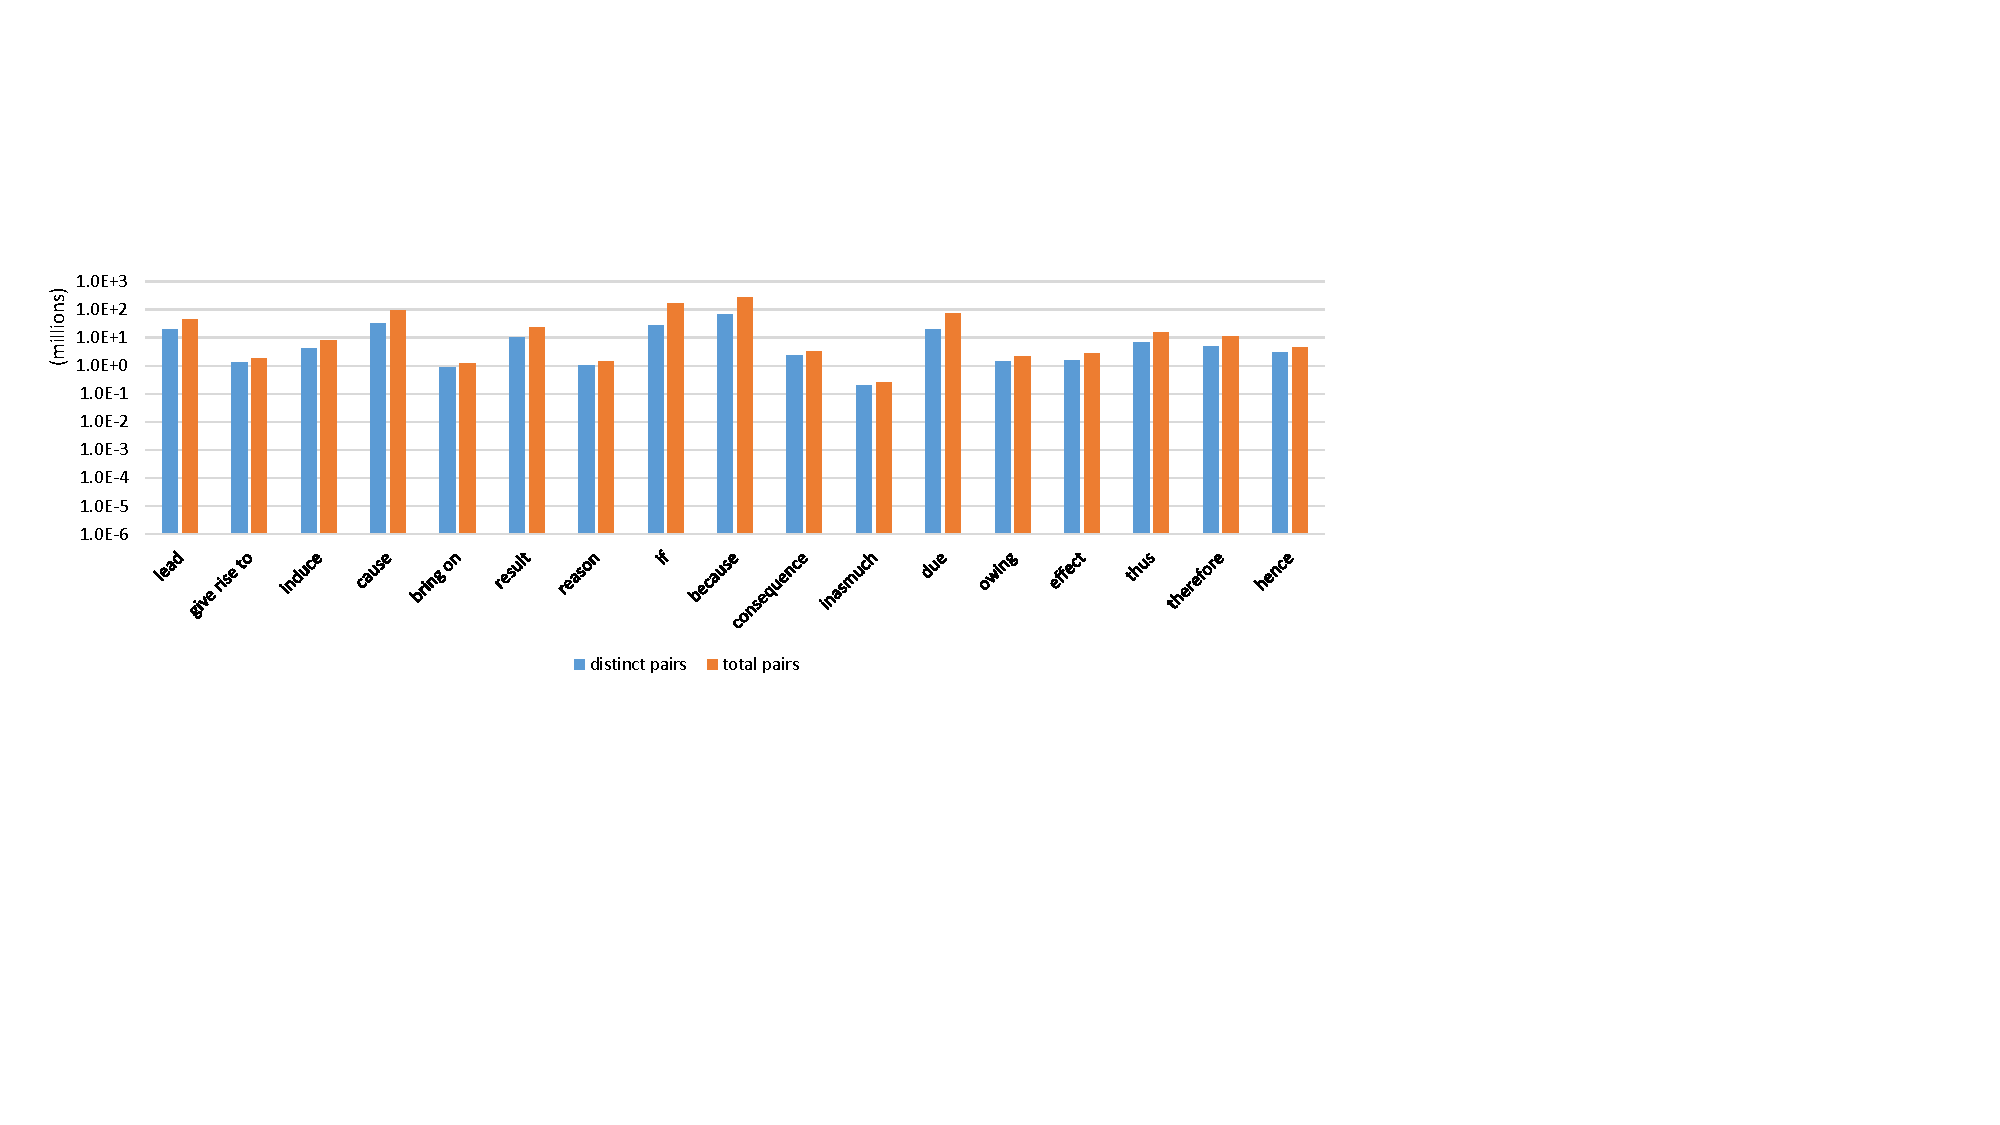
\includegraphics[width=2\columnwidth]{pattern.pdf}
\caption{Number of causal vs. non-causal pairs from ConceptNet covered by cues}
\label{fig:pattern2}
\end{figure*}

To evaluate the quality of the causal cues, we make use of the
manually labeled causal events in
ConceptNet~\cite{liu2004commonsense} as ground truth. ConceptNet 4
contains 74,336 unlemmatized English words, forming
375,135 unique concepts, which are connected by 610,397 relation edges.
Only some of these relations encode causal knowledge,
such as ``Causes'', ``CausesDesire'' and ``HasPrerequisite''.
The total number of such causal relation is 52778.
This is significantly smaller than our
CausalNet in scale, especially in terms of number of edges.
%Otherwise, relations are more sparse in ConceptNet.
We randomly collect 100 causal even pairs and 100 non-causal event pairs from
ConceptNet,
based on feedbacks from human volunteers of OMCS project, who cast positive
votes for each \emph{Causes} relationship that is causal, and
negative for that is not. Since the pairs from ConceptNet contain
phrases and not just words, we consider a pair ($x$, $y$) to be covered by a
causal cue, if at least one word $u$ from $x$ and another word $v$ from
$y$ are extracted as cause word and effect word by the cue
from the web corpus.
\figref{fig:pattern2} shows that in general, our cues can
effectively distinguish between positive and negative causal pairs,
with the exception of ``hence'' and ``consequence'', both of which
represent relatively coarse-grained entailment relation.
Particularly good cues to distinguish the positive and negative
pairs are ``due to'' and ``induce''.

%[optional: Figure 2 is the top-ranked results after considering idf weight for
%each term.]

%\begin{figure*}[htp]
%\centering \scalebox{0.5}{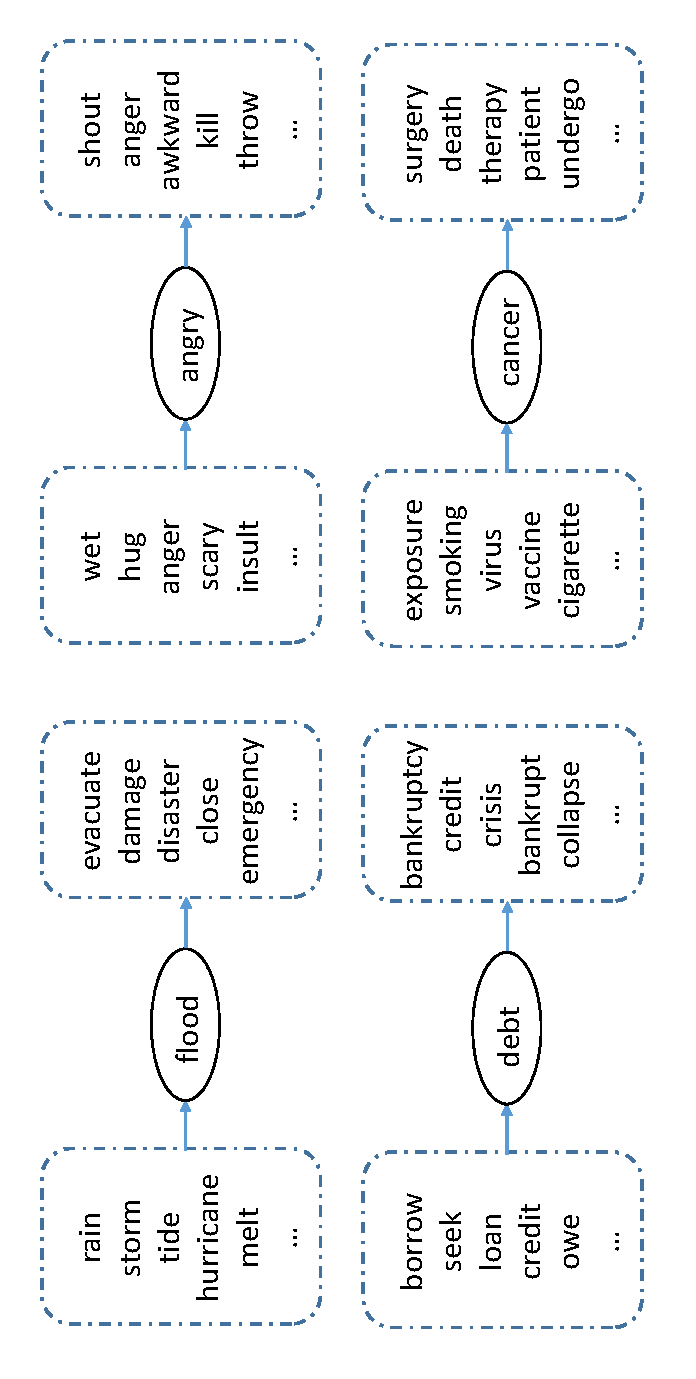
\includegraphics[angle=270,clip]{111.eps}}
%\caption{Concrete examples of CausalNet demo}
%\label{fig:example1}
%\end{figure*}

%1. zoom into demo, show some examples and analysis of
%our graph Figure
%A Snapshot of CausalNet

%==[optional] next, we can show a figure that is ranked by idfweight*causal
%strength ==


\subsection{End-to-end Evaluation on COPA}
COPA task consists of 1000 causal reasoning questions, divided into
development question set and test question set of 500 each.
The authoring methodology of COPA ensured sufficient breadth of the topics
in the question set. Each question in COPA data set was validated
by two raters with high inter-rater agreement.
In addition, the incorrect alternative was purposely set semantically
close to the premise, which makes this task more difficult for
purely associative methods.

We tuned the parameters $\alpha$ and $\beta$ on the development set by
attempting all combinations of values from 0 to 1.0 with a step of
0.1. The best combination was empirically found  to be $\alpha=0.4$,
$\beta=0.3$. Note that, setting parameter $\alpha=0$,
$\beta=0$ models the causal strength to be exactly the product of
two conditional probabilities. Another extreme would be setting
$\alpha=1$, $\beta=1$, where the causal strength becomes \eqnref{eq:pmi2},
which is actually the square of PMI with causal directions
itself without logarithm.
%Our method without event enhancement
%serves as a baseline; it does not detect any events or
%boost the strength of any word in the
%input sentence but merely uses the causal network and the
%causal strength scores between words.

We compare our system (with and without event enhancement step)
with a number of state-of-the-art systems, and report the results in
\tabref{tab:evaluation}.
All competing systems were assessed based
on their accuracy on the 500 questions in the COPA test
split~\cite{gordon2012copa}.

%but we also show the accuracy on development set and all questions.
%The overall score is the mean value of development and test set because the two
% sets have equal number of examples.
%Table~\ref{tab:evaluation}
%\begin{table}[th]
%\small
%\centering
%\caption{COPA results comparison}
%\begin{tabular}{|l|c|c|c|}
%\hline Methods & Dev & Test & All  \\ \hline \hline
%PMI Gutenberg (W=5)\cite{roemmele2011choice} & 57.8\% & 58.8\% & 58.3\% \\
%UTDHLT Bigram PMI\cite{goodwin2012utdhlt} & - &61.8\% & - \\
%UTDHLT SVM Combined\cite{goodwin2012utdhlt} & - &63.4\% & - \\
%PMI 10M Stories (W=25)\cite{gordon2011commonsense} & 62.8\% & 65.4\% & 64.1\%
% \\ \hline CausalNet without Events &62.8\%& 67.6\% & 65.2\%  \\
%{\bf CausalNet with Events} &62.8\% & {\bf 68.8} \% & {\bf 65.8}\%  \\
%\hline
%\end{tabular}
%\label{tab:evaluation}
%\end{table}

\begin{table}[th]
%\small
\centering
\caption{COPA results comparison}
\label{tab:evaluation}
\begin{tabular}{lccc}
\hline
Methods & Accuracy(\%) \\
\hline
PMI Gutenberg (W=5)\cite{roemmele2011choice}  & 58.8\% \\
PMI Gutenberg (W=25)\cite{roemmele2011choice}  & 58.6\% \\
UTDHLT Bigram PMI\cite{goodwin2012utdhlt} &61.8\% \\
UTDHLT SVM Combined\cite{goodwin2012utdhlt} &63.4\% \\
%PMI 1M Stories ()
PMI 1M Stories (W=25)\cite{gordon2011commonsense} & 65.2\% \\
PMI 10M Stories (W=25)\cite{gordon2011commonsense} & 65.4\% \\ \hline
%\ZY{PMI 10TB web corpus (W=xx)} & \ZY{xxx}\% \\
CausalNet w/o events & 67.6\%  \\
{\bf CausalNet w/ events} & {\bf 68.8} \%   \\
\hline
\end{tabular}
\end{table}

PMI Gutenberg uses PMI statistic calculating from data in Project
Gutenberg (16GB of English-language text). They pair the words from
premise and alternative and choose the alternative with a higher
PMI. Their result is the best with a window size of 5. UTDHLT is the
result of SemEval-2012 Task 7 systems. This team proposes two
approaches for the task. The first one uses PMI over bigrams as a
feature. For the second one, they treat it as a classification
problem and combine the features used in the first approach  with
some additional features to train an SVM model. Their PMI statistic
is calculated from the LDC Gigaword corpus (8.4 million documents).
%The author only provides the score of test set such that results for
% development and all set could not be reported.
 The last PMI method, which was also the best
performing method in the last 4 years, uses a larger corpus of
personal stories (37GB of text) with a window of 25.
Observe that our system with the event detection and
boosting in \secref{sec:eventBoost}, shown in bold, achieves
$68.8\%$ and outperforms all existing approaches.


To answer the question whether it is the large corpus size or the
effectiveness of our algorithm that contributes to the better
results in our approach, we implement Gordon's PMI
method\cite{gordon2012copa} on our own web corpus. We applied
different window-size parameter to Gordon's PMI method and compare
their results on COPA with ours again in \tabref{tab:baseline}.

\begin{table}[th]
%\small
\centering
\caption{COPA results for PMI method on web corpus}
\label{tab:baseline}
\begin{tabular}{lc}
\hline
System & Accuracy(\%) \\
\hline
PMI 10T web corpus(W=5) & 61.6\% \\
PMI 10T web corpus(W=10) & 61.0\% \\
PMI 10T web corpus(W=15) & 60.4\% \\
PMI 10T web corpus(W=25) & 61.2\% \\
\hline
CausalNet w/o events & 67.6\%  \\
{\bf CausalNet w/ events} & {\bf 68.8} \%   \\
\hline
\end{tabular}
\end{table}

The differences in accuracy between ours and Gordon's PMI are
statistically significant at $p<0.05$, \footnote{Statistical
significance in this paper is calculated using stratified shuffling
\cite{resampling1989computer}.} both with and without event
enhancements. Our system using the same web corpus significantly
outperforms the best PMI-based result, which validates the
effectiveness of our framework, and not the scale, makes such
difference.

By comparing \tabref{tab:evaluation} and \tabref{tab:baseline},
we echo the view from \cite{gordon2011commonsense} that specialized
personal story corpus is useful for causality detection.
However, the size of such corpus is nowhere near the size of a generic
web corpus.
The contribution of our approach is that it does a better job at
leveraging a much bigger but more general web
corpus, in place of specialized corpus with limited availability.

% \ZY{\subsection{Supplementary Experiments}}
%
% \begin{figure}[th]
% \centering
% \epsfig{file=gu_pmi_1.eps, width=\columnwidth}
% %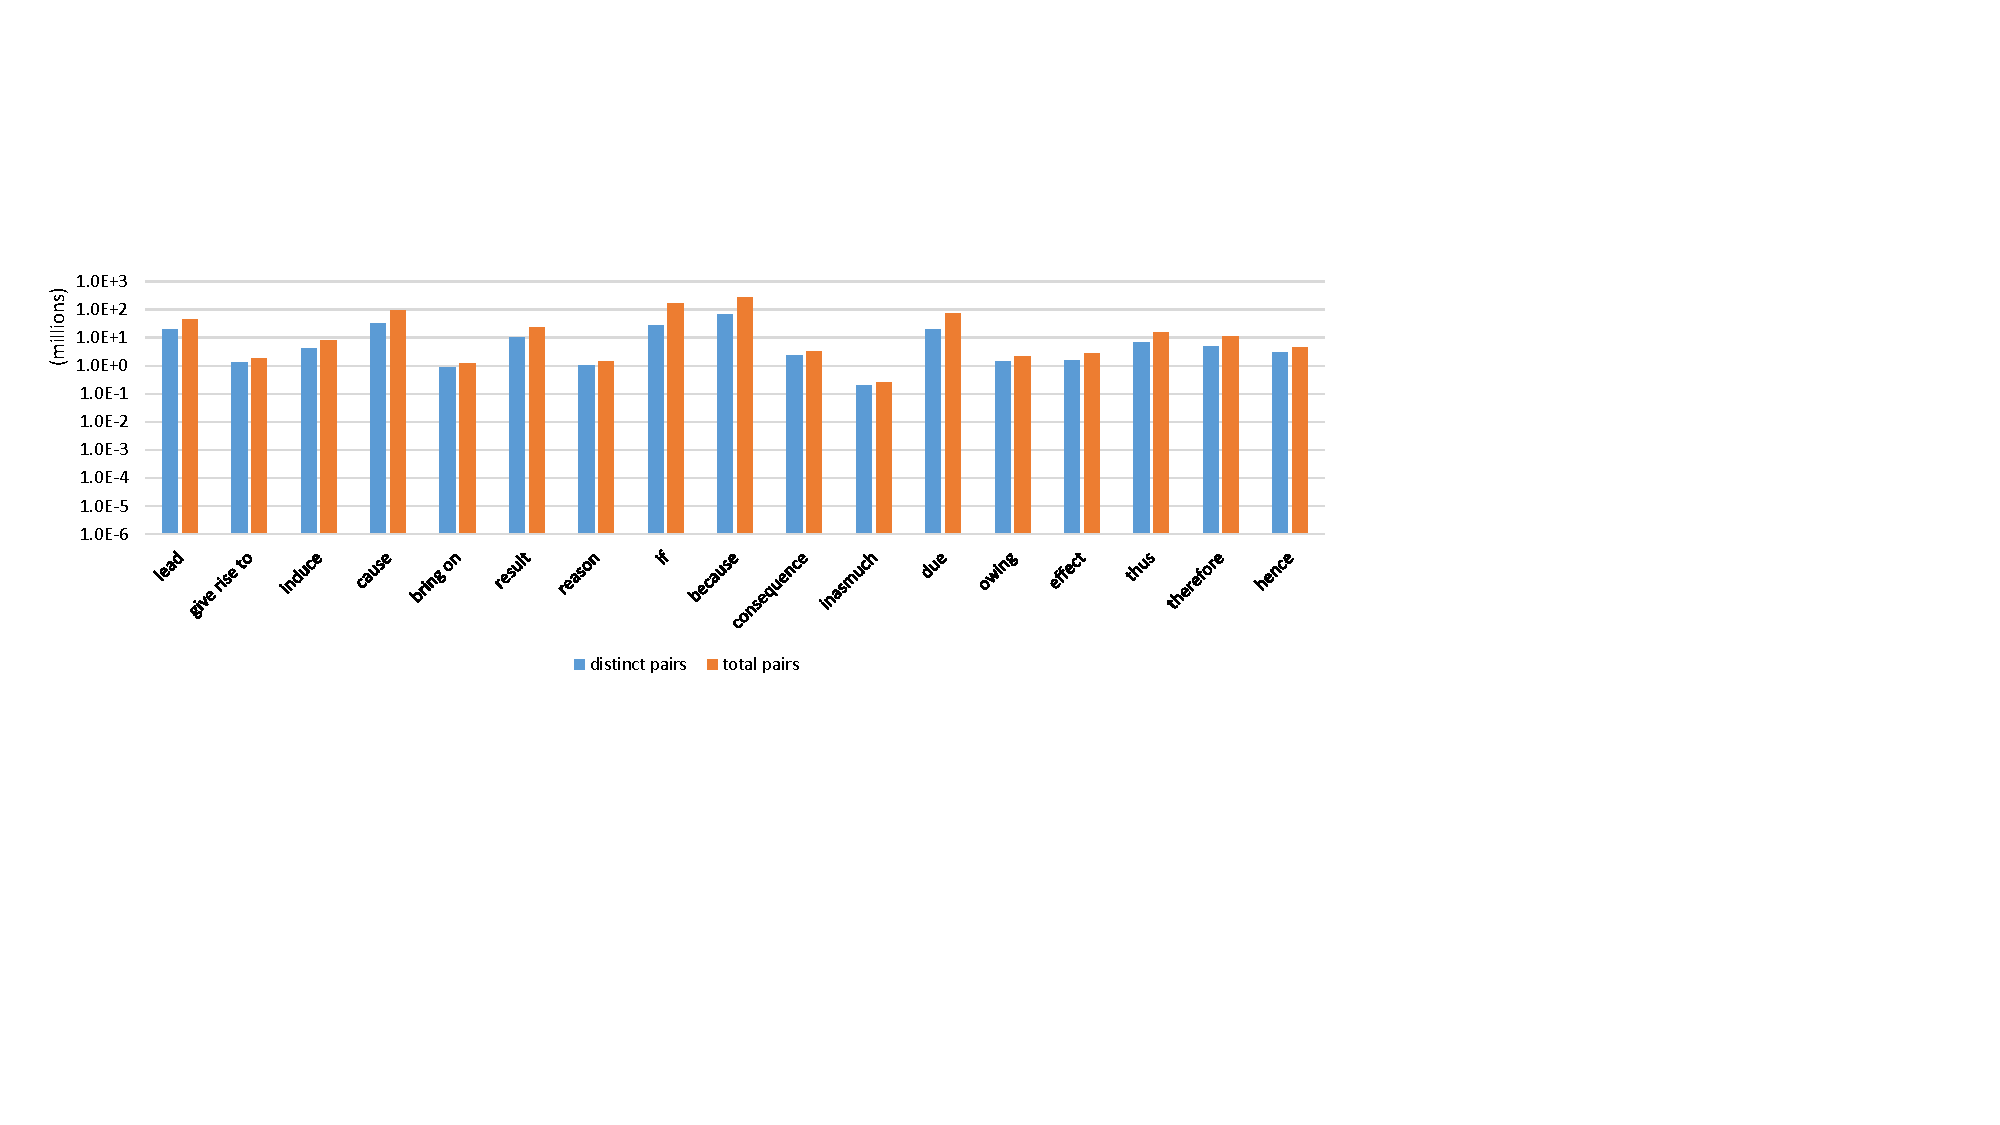
\includegraphics[width=2\columnwidth]{pattern.pdf}
% \caption{COPA Results by varying corpus size of Gutenberg }
%
% \label{fig:gu_pmi_1}
% \end{figure}

\subsection{Causality Detection}

Causality detection is another relevant application to our
work. Identifying the causal relation in text is an important task
for many applications, such as event prediction, risk analysis, or
decision making support\cite{mirza2014extracting}. To show the
effectiveness of our work in this aspect, we investigate the
following two research questions on our proposed network, using data
from ConceptNet4.
\begin{itemize}
\item {\bf RQ1:}
For arbitrary event pair manually labeled as \emph{causal} (positive data)
or \emph{non-causal} (negative data), we investigate whether our
proposed causality score clearly separates the two.
\item {\bf RQ2:} Inspired by COPA, we select causal and non-causal pairs
sharing the same premise from ConceptNet and form two-choice
questions, to evaluate the ability of CausalNet in selecting the
correct choice.
\end{itemize}

%More specifically,
%we use \emph{pseudo-disambiguation task} used in~\cite{Erk}.
%Intuitively, ConceptNet, being manually generated, is limited in coverage,
%but expected to be near-perfect in precision.
%In particular, we follow Erk to use
%near-perfect causal event pairs $(u,v)$ from ConceptNet as positive ground-truth
%for testing, and to pair $u$
%with another random instance $v$ as negative ground-truth instances.

%The task is then to choose more likely effect $u$ among $v$ and $v'$
%using our network.
%(We can report precision and recall, and high score
%indicates that we are as good as ConceptNet in detection, with XX times larger
%coverage.
%Maybe we can show some pairs we found, as in your EMNLP draft if we are proud.)


For {\bf RQ1,}
%We do two applications based on ConcpetNet to show both reasonable of our
%causality metric on global causal pairs (thought it is difficult to give a
%threshold for causal relationship identification task) and usefulness to select
%plausible cause/effect from multiple-choice.
we use the same 200 causal and non-causal event pairs from
\figref{fig:pattern2} as positive and negative data.
%\ZY{For the ``Causes'' relation in
%ConcpetNet, people votes +1/-1 for event pairs in terms of particular relation
% to show their tendency whether the particular relation exists in the pair.
%The pairs with high positive votes (more than 3 in our experiment) in terms of
% ``Causes'' relation can be seen as positive examples, as those pairs with negative votes can be seen as negative examples.} Figure
\figref{fig:conceptApp1} shows the causality score ($y$-axis) of 100 positive
and negative pairs indexed randomly ($x$-axis). We can observe that scores
of positive and negative pairs are accurately distinguished by a
linear function, such as $y=10^{-2}$, indicated by the green line,
with little overlap. Consequently, existing systems that aim at
causality identification and detection can incorporate
our work to improve their accuracy.

\begin{figure}[htb]
\centering
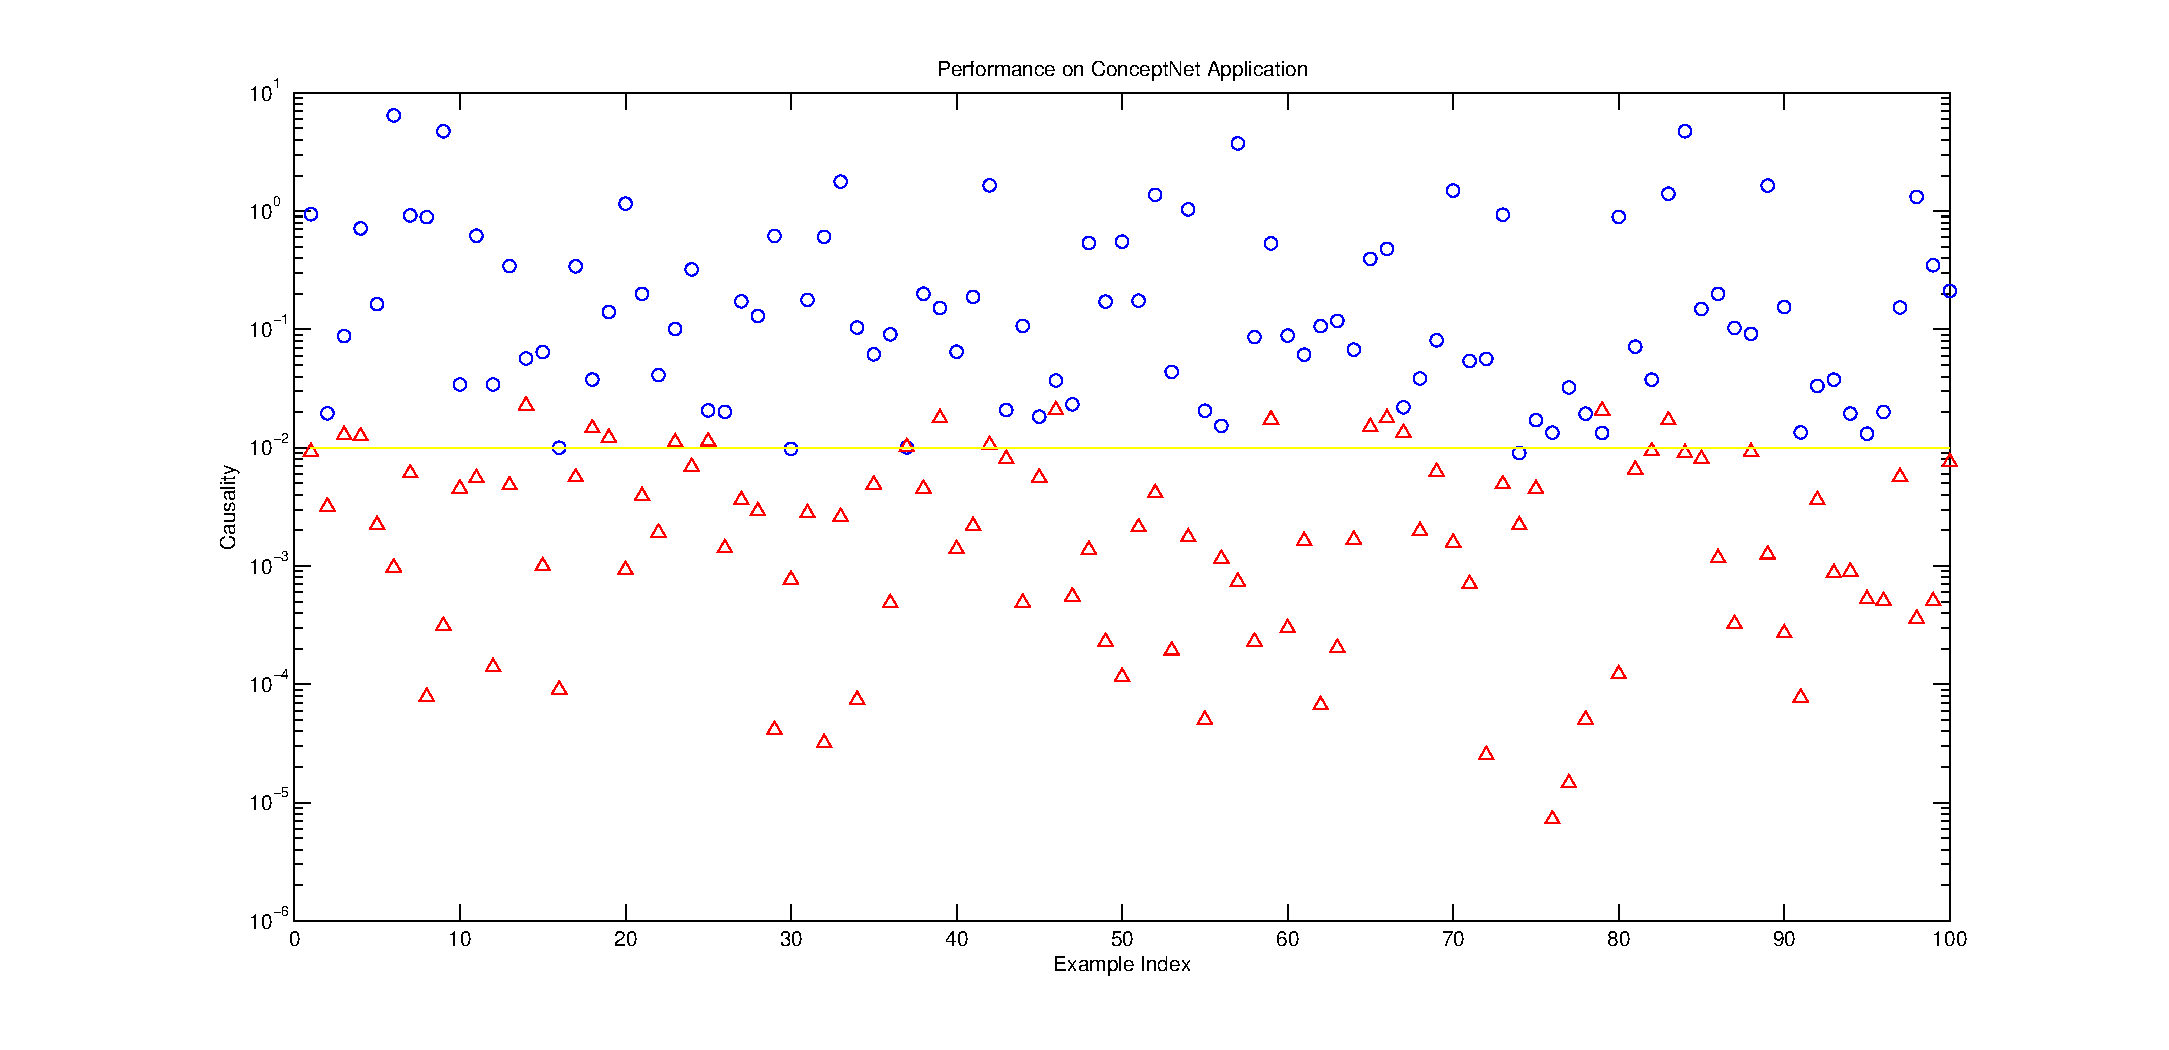
\epsfig{file=conceptApp1.eps, width=0.8\columnwidth}
\caption{Distinguishing causality on ConceptNet}
\label{fig:conceptApp1}
\end{figure}

For {\bf RQ2,} we test our network in a COPA-like setting
of classifying between causal and non-causal pairs sharing the
same premise. Due to sparsity of such pairs,
we follow \emph{pseudo-disambiguation task} in~\cite{Erk}.
%Intuitively, ConceptNet, being manually generated, is limited in coverage,
%but expected to be near-perfect in precision.
In particular, we use \emph{Causes} relationship $(u,v)$ with
positive votes, such that $u$ is the shared premise and $v$ is a
positive alternative. We then generate a negative alternative by
randomly selecting $v'$ without \emph{Causes} relationship with $u$.
This approach is widely adopted in many tasks, as a large scale test
cases can be generated, but as ConceptNet does not exhaustively
label all possible causal relationships, randomly selected $v'$ can
be actually causal, or \emph{false negatives} may exist. In such
situation, we removed the question involving such false negative,
and consequently obtained a dataset of 412 questions in which 259
look for an effect while 153 look for a cause. \tabref{tab:rq2}
shows that the system with event enhancement outperforms the one
without.

\begin{table}[th]
%\small
\centering
\caption{Result of ConceptNet RQ2}
\begin{tabular}{cc}
%\hline CausalNet w/ events & CausalNet w/o events   \\ \hline \hline
\hline
Methods & Accuracy(\%) \\
\hline
CausalNet w/o events & 78.4\%  \\
{\bf CausalNet w/ events} & {\bf 80.1\% }  \\
\hline
\end{tabular}
\label{tab:rq2}
\end{table}

\subsection{Direction of Causality}
%
%Causal relation is one form of relatedness. Thus,
%identifying a subset of causality from general relatedness is a
%challenge task. This section evaluates such ability of CausalNet via
%investigating its effectiveness of causality directional prior,
%since relatedness is a symmetric relation and causality is
%asymmetric.
%
Given a pair of terms $u$ and $v$ that are causally related,
CausalNet can generally tell whether the causality is encoded by $u
\rightarrow v$ or by $v \rightarrow u$, without the context of
$u$ and $v$. In other words, as we will show next, CausalNet
provides a reasonable prior knowledge of causality direction.
We use the annotated corpus of SemEval-2010 Task 8 to evaluate this.
There are 920 pairs of terms annotated as Cause-Effect relationship in
SemEval-2010 Task 8 training corpus. CausalNet covered 894 out of
920 pairs (97.2\%). Each Cause-Effect pair in the SemEval data set is
annotated as follows:
\begin{itemize}
  \item[] Sentence:\\
  \emph{I too, get a <e1>\textbf{headache}</e1> from
  <e2>\textbf{wine}</e2>, and was always told that it was the sulfites.}
  \item[] Relation: \\ \emph{Cause-Effect($e2$,$e1$)}
\end{itemize}
In the above example, $e1$ represents the term ``headache'', and
$e2$ represents ``wine''. The relation Cause-Effect($e2$,$e1$)
indicates that the causality encoded in this sentence is
\emph{wine}$\rightarrow$ \emph{headache}, but not
\emph{headache}$\rightarrow$ \emph{wine}. We can obtain this useful
insight by the commonsense from CausalNet.
We simply compare the causal strength of
$u \rightarrow v$ with that of $v \rightarrow u$ provided by
CausalNet. If $CS(u \rightarrow v) > CS(v \rightarrow u)$, we
believe that the causality is encoded by $u \rightarrow v$,
otherwise the causality is encoded by $v \rightarrow u$.

The agreement between CausalNet and annotated ground truth in SemEval-2010
Task 8 is 82.3\%, that is 736 out of 894 pairs from SemEval find a matching
pair in the same causal direction from CausalNet.
\tabref{tab:sample} shows 40 random samples of annotated causal pairs
from SemEval-2010 Task 8 corpus. 20 of those are matched by
CausalNet and the other 20 are not. Three human judges were employed to
mark whether these pairs follow common sense or not. Those italicized pairs
are considered common sense by at least 2 judges.
We can see that all but one pairs in the left column are common sense,
while most of those pairs in the right column are not common sense.
This means, where CausalNet predicts correctly, it is really due to the power
of commonsense knowledge. On the other hand, CausalNet makes mistakes primarily
due to the lack of context in small amount of cases, and not because the
knowledge enclosed is wrong.

\begin{table}[th]
\centering
\caption{Random samples of annotated causal pairs from SemEval-2010 task 8}
\label{tab:sample}
\small
\begin{tabular}{|c c | c c |}
\hline \multicolumn{2}{|c|}{Pairs with match in CausalNet} &
\multicolumn{2}{c|}{Pairs without match in CausalNet}\\
%\hline intra-sentence cue & inter-sentence cue  \\
\hline \hline
\multicolumn{1}{|c}{Cause} & \multicolumn{1}{c|}{Effect} & \multicolumn{1}{|c}{Cause} & \multicolumn{1}{c|}{Effect} \\
\hline
%\hline & \\
%\hline &\\
%A cause B & B caused by A & A induce B & If A, then B & A, hence B & A, thus B\\

\emph{vaccine} & \emph{fever}    & \emph{drink} & \emph{suffering} \\
\emph{tension} & \emph{headache}     & malfunction & inflammation\\
\emph{passage} & \emph{noise}    & growth & inflammation\\
\emph{injury} & \emph{discomfort}    & pie & poison\\
ash & drama  & city & anger\\
\emph{press} & \emph{reaction}   & \emph{infection} & \emph{acne}\\
\emph{extraction} & \emph{extinction}    & institution & fraud\\
\emph{mess} & \emph{crisis}  & dog & joy\\
\emph{pinworm} & \emph{infestation}  & fear & attack\\
\emph{parasite} & \emph{toxoplasmosis}   & \emph{bacteria} & \emph{acne}\\
\emph{disability} & \emph{benefit}   & \emph{fireplace} & \emph{warmth}\\
\emph{elimination} & \emph{riot}     & tax & fluctuation\\
\emph{generator} & \emph{signal}     & \emph{bacteria} & \emph{breakout}\\
\emph{drug} & \emph{unconsciousness}     & \emph{injury} & \emph{operation}\\
\emph{zinc} & \emph{growth}  & \emph{pregnancy} & \emph{nausea}\\
\emph{reaction} & \emph{inversion}   & \emph{attack} & \emph{shock}\\
\emph{movement} & \emph{earthquake}  & lack & reliance\\
\emph{virus} & \emph{disease}    & computer & radiation\\
\emph{drum} & \emph{sound}   & ointment & discomfort\\
\emph{vaccine} & \emph{outbreak}     & ginseng & taste\\
\hline
\end{tabular}
\end{table}

%CausalNet provides pretty (pretty?) good prior knowledge for commonsense
%causality, since we do not use other local context information.
%This shows that CausalNet can effectively tell the difference
%from relatedness and causality.

\begin{figure*}[th]
\centering
\begin{subfigure}[t]{0.9\columnwidth}%0.7\columnwidth
\centering
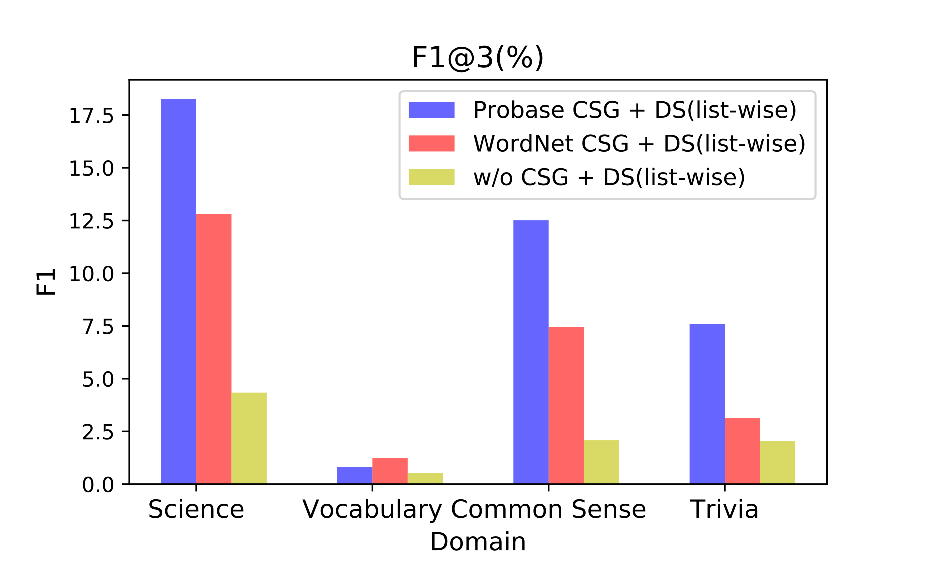
\epsfig{file=f1.eps, width=0.9\columnwidth, angle=0,
clip}%width=0.4\columnwidth, angle=270
\caption{flood}
\end{subfigure}
\begin{subfigure}[t]{0.9\columnwidth}
\centering
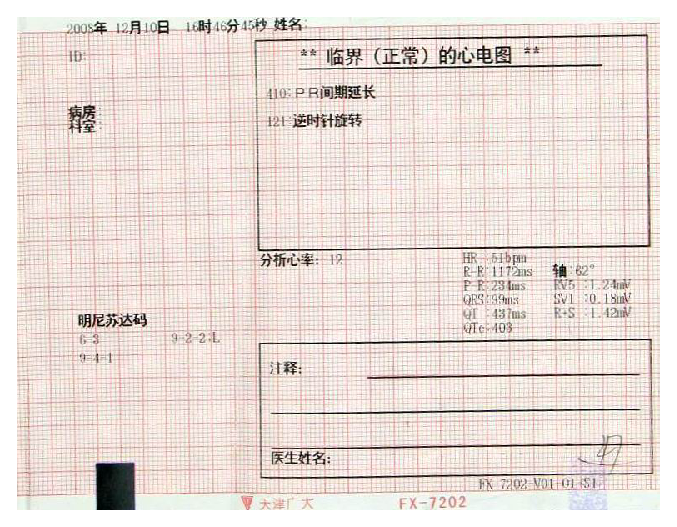
\epsfig{file=f2.eps, width=0.9\columnwidth, angle=0, clip}
\caption{cancer}
\end{subfigure}
\begin{subfigure}[t]{0.9\columnwidth}
\centering
\epsfig{file=f3.eps, width=0.9\columnwidth, angle=0, clip}
\caption{debt}
\end{subfigure}
\begin{subfigure}[t]{0.9\columnwidth}
\centering
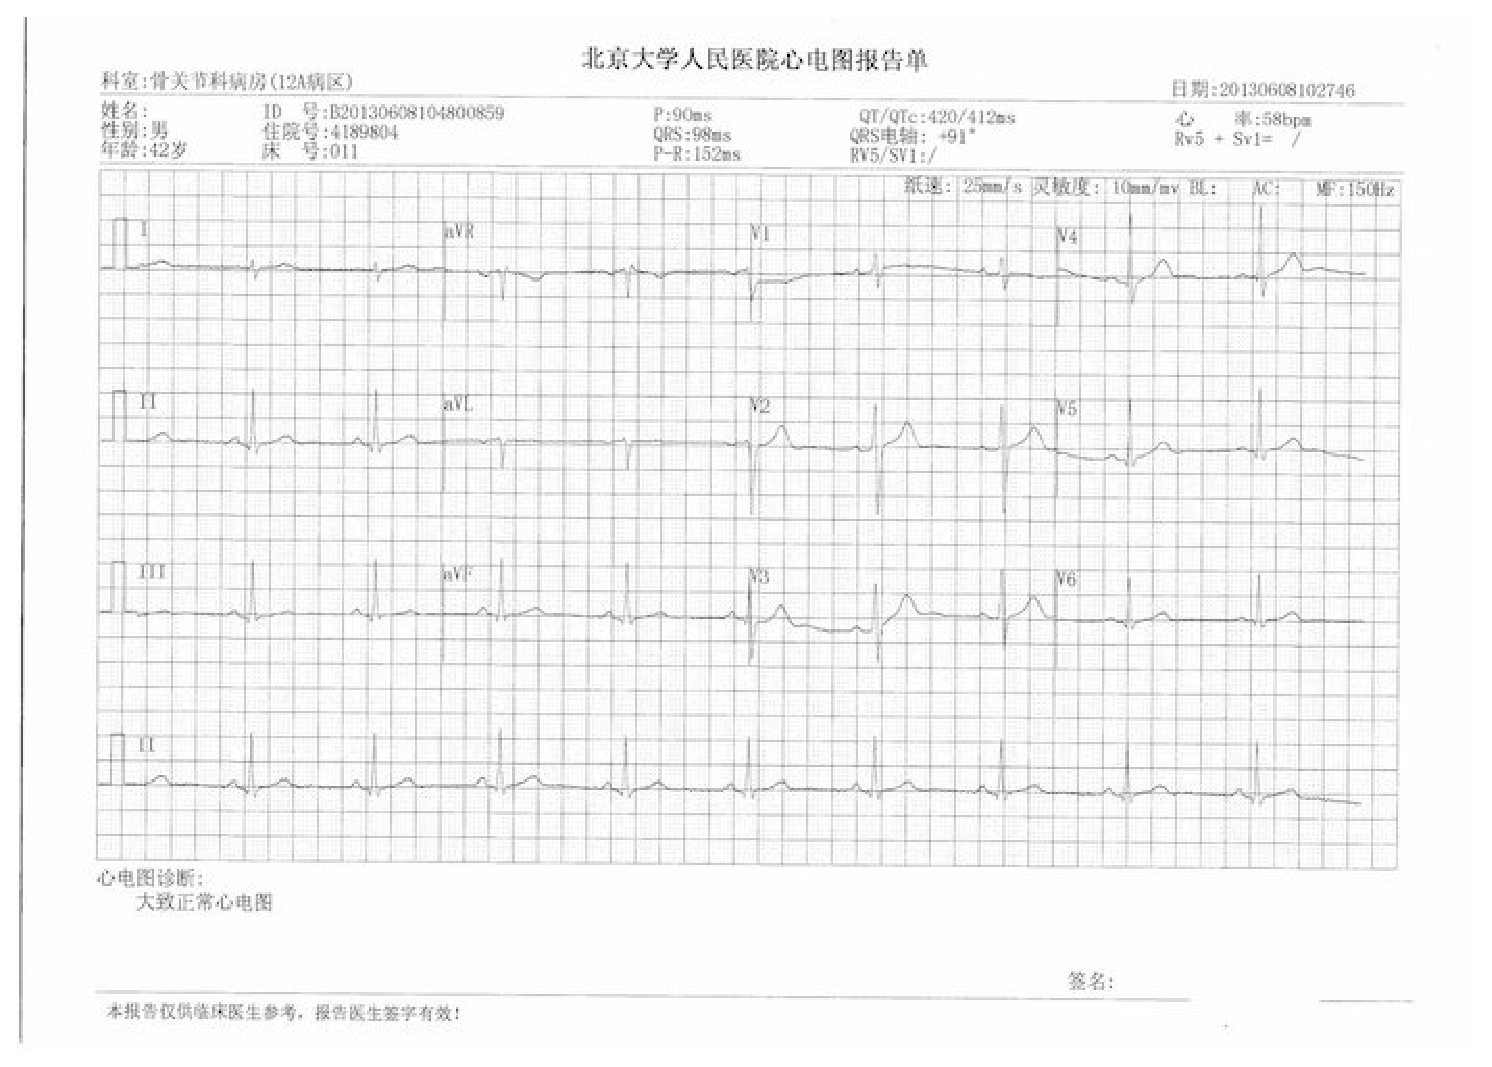
\epsfig{file=f4.eps, width=0.9\columnwidth, angle=0, clip}
\caption{angry}
\end{subfigure}
\begin{subfigure}[t]{0.9\columnwidth}
\centering
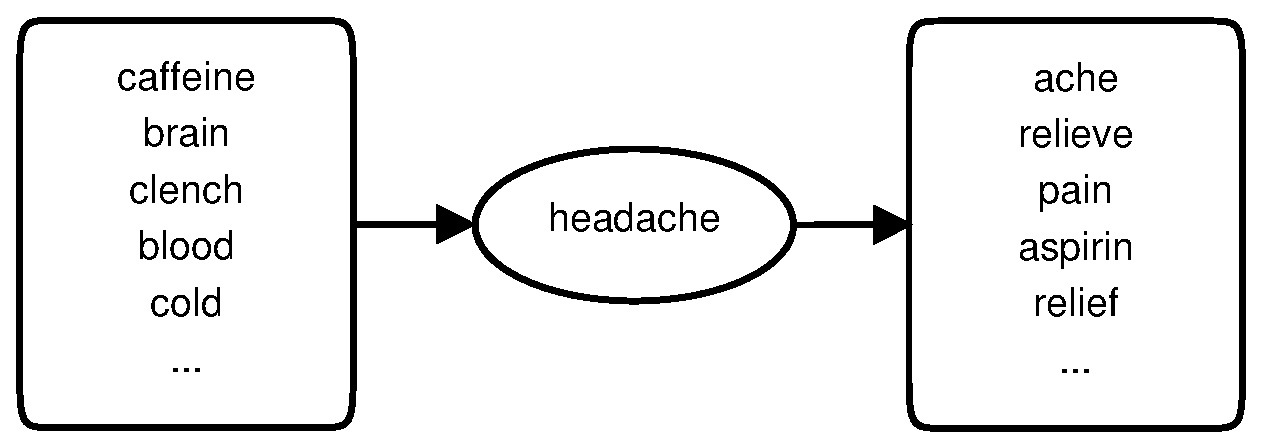
\epsfig{file=f5.eps, width=0.9\columnwidth, angle=0, clip}
\caption{headache}
\end{subfigure}
\begin{subfigure}[t]{0.9\columnwidth}
\centering
\epsfig{file=f6.eps, width=0.9\columnwidth, angle=0, clip}
\caption{guilty}
\end{subfigure}
%
%\subfigure[]{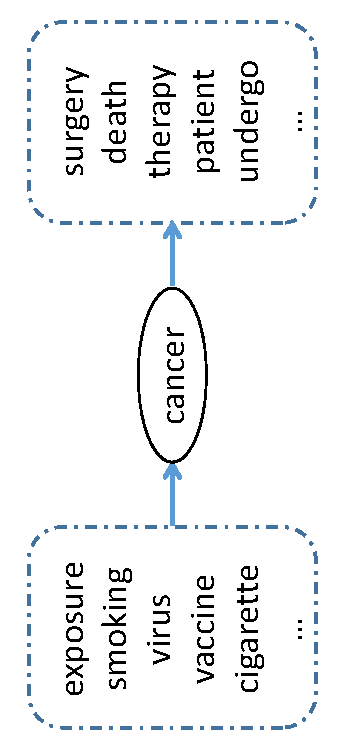
\epsfig{file=ex2.eps, width=0.25\columnwidth, angle=270, clip}}
%\subfigure[]{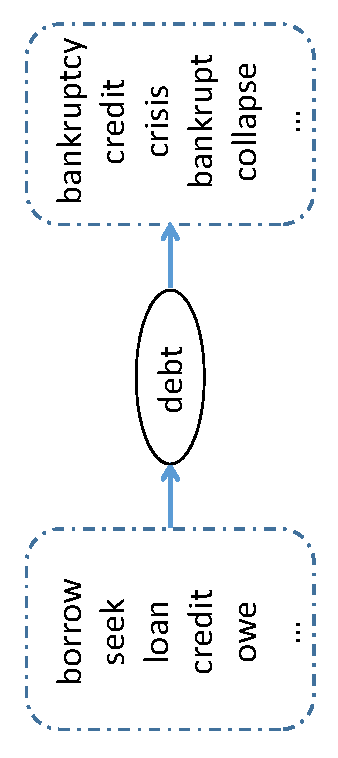
\epsfig{file=ex3.eps, width=0.25\columnwidth, angle=270, clip}}
%\subfigure[]{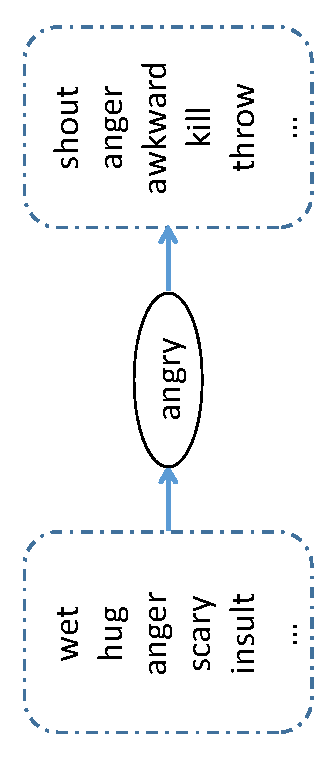
\epsfig{file=ex4.eps, width=0.25\columnwidth, angle=270, clip}}
%\subfigure[]{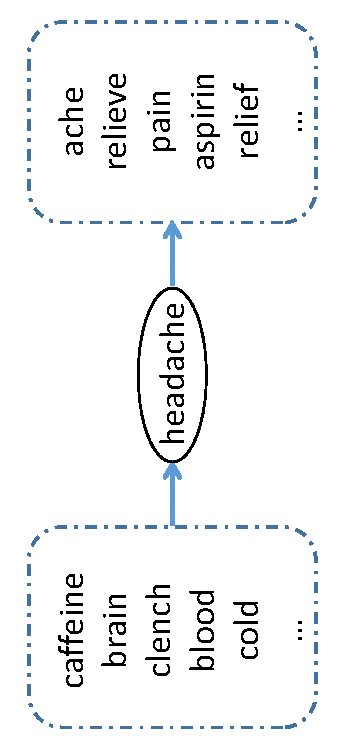
\epsfig{file=ex5.eps, width=0.25\columnwidth, angle=270, clip}}
%\subfigure[]{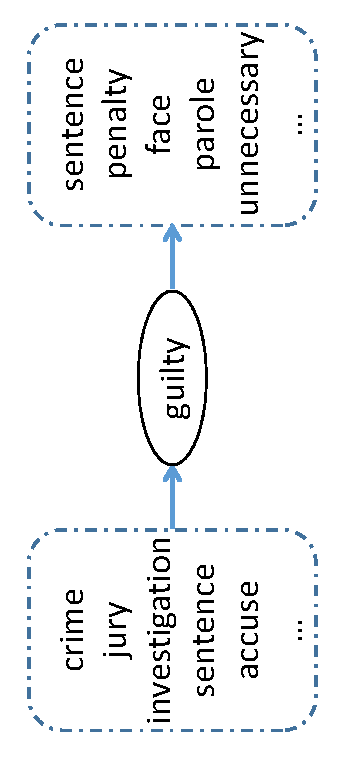
\epsfig{file=ex6.eps, width=0.25\columnwidth, angle=270, clip}}
%\subfigure[]{\scalebox{0.42}{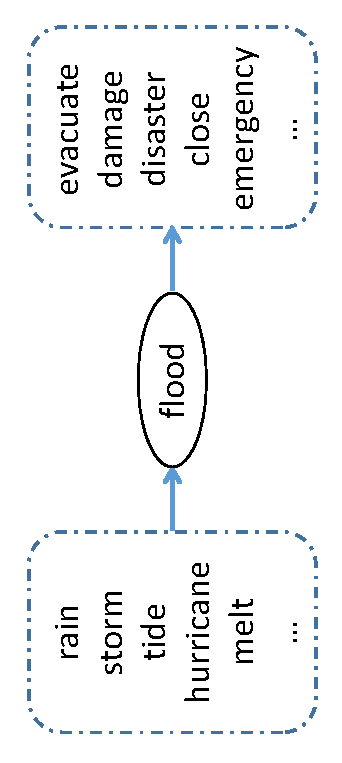
\includegraphics[angle=270,clip]{ex1.eps}}}
%\subfigure[]{\scalebox{0.42}{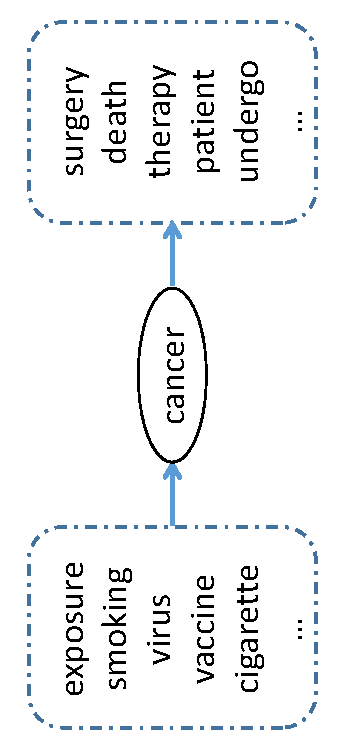
\includegraphics[angle=270,clip]{ex2.eps}}}
%\subfigure[]{\scalebox{0.42}{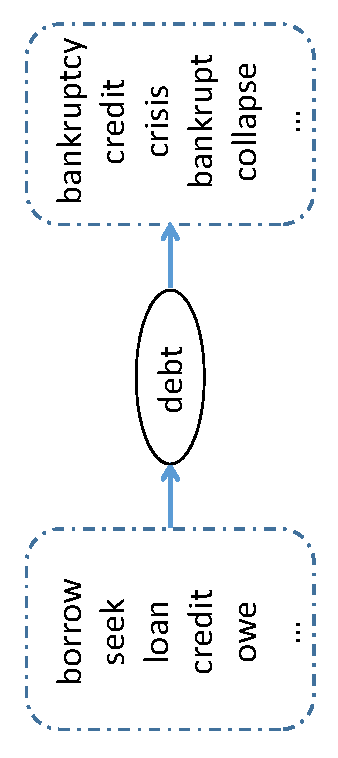
\includegraphics[angle=270,clip]{ex3.eps}}}
%\subfigure[]{\scalebox{0.42}{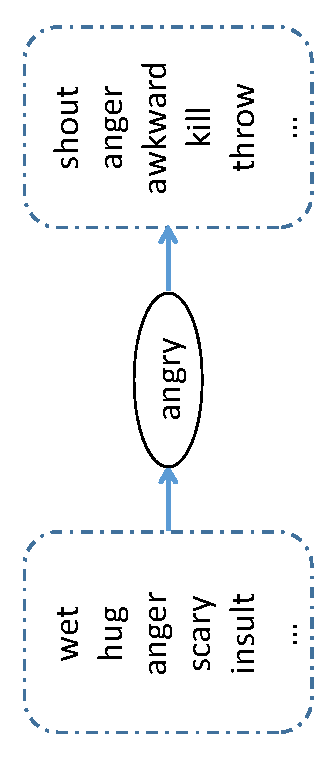
\includegraphics[angle=270,clip]{ex4.eps}}}
%\subfigure[]{\scalebox{0.42}{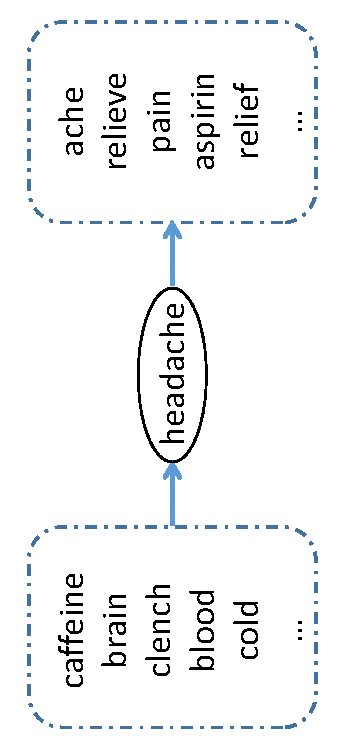
\includegraphics[angle=270,clip]{ex5.eps}}}
%\subfigure[]{\scalebox{0.42}{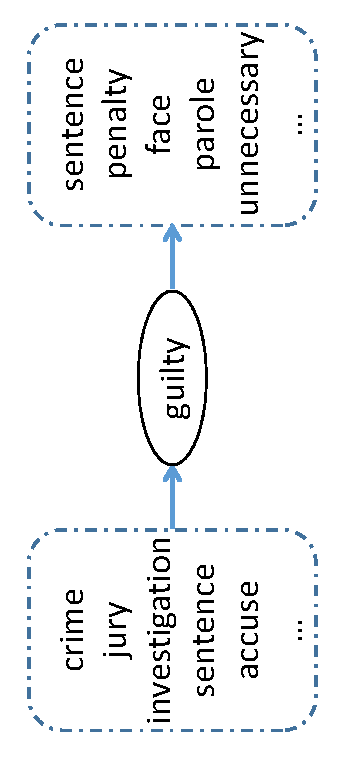
\includegraphics[angle=270,clip]{ex6.eps}}}
\caption{Examples from CausalNet demo}
\label{fig:example1}
\end{figure*}



%More examples of ConceptNet (and a complete ranking of causal words)  can be
%found from \url{http://202.120.38.146/causal/causalnet.html} ,

\subsection{Demo and Discussion}
\label{sec:discuss}
\begin{figure}[th]
\centering
\epsfig{file=snapshot.eps,width=\columnwidth}
\caption{A snapshot of the demo}
\label{fig:snapshot}
\end{figure}

The complete demo includes 2881 unique lemmatized words that ever appear
in the COPA data set. Stanford NLP tools \cite{chen2014fast} were used for
lemmatization. Topics in COPA data set were drawn from
different sources\cite{roemmele2011choice} to ensure comprehensive coverage
of different domains.
% want to show some results and talk about existing issues in our work
To further illustrate CausalNet, we give some concrete
examples from our demo (with a snapshot shown in \figref{fig:snapshot}).
Arrows shown in
\figref{fig:example1} indicate the directions of causality.
\figref{fig:example1} (a),(b),(c),(d),(e) and (f) show the top 5 ranked
causes and effects of the terms, ``flood'', ``cancer'', ``debt'',
``angry'', ``headache'', and ``guilty'', respectively.

Capturing commonsense causal relations for all words is
an ambitious goal.
While CausalNet generally gives reasonable causes and effects
for most common words,
there are still noises and errors.
%Our end-to-end COPA evaluation accuracy is still below 70\%.
For example, in \figref{fig:example1} (d), ``wet'' and ``hug'' rank ahead of
``insult'' as the causes of ``angry'', which is counter-intuitive to most
people.
%This section we show analysis our extracted commonsense causal knowledge.
% Although, we introduced techniques to solve
%It's really a challenging task to get pretty robust causality ranking
%results. As \figref{fig:example1} (d) shown, the term ``wet'' ranks higher than
%``insult''.
%CausalNet is inevitably biased toward terms with high popularity in
%common sense. Relative reasonable results are acceptable
%for commonsense causal reasoning.
Our preliminary analysis shows that these noises and errors are due to
two limitations of our approach.

First, CausalNet is constructed on individual words only, but many events
cannot be effectively encoded in a single word. For example, our investigation
shows that \emph{hug} $\rightarrow$ \emph{angry} in \figref{fig:example1} (d)
is likely extracted from patterns such as
``because...refuse to hug, ... angry''. In fact, our extracted pair
 \emph{hug} $\rightarrow$ \emph{angry} is only part of a ``negative''
causal relation $not~ hug \rightarrow angry$. Fortunately, while some
of the causal word pairs from CausalNet do not appear very rational in their
own right, when used with other pairs together,
the combined causal strength can provide
reasonable commonsense reasoning between more complex text units.

Second, pattern-based extraction has its limitation.
The 53 causal cues we used to extract CausalNet are indicative of
a potential causal relation in the text. But this is not always true.
For example, ``$A$ rarely causes $B$'' matches one of the cues but is certainly
not causality. This kind of situation gives rise to many false positives in
CausalNet. Furthermore, causal cues do not capture implicit causality.
People may say ``I'm not hungry, I just had lunch.'' instead of
``I'm not hungry because I just had lunch.'' Such implicit causal knowledge
is currently ignored by our approach.
Existing approaches, such as \cite{ittoo2011extracting}, attempted to
obtain implicit causality on domain-specific texts.
But such work can not easily extend to open
domain causality acquisition due to the introduction of excessive noise.
%More efforts need to be done on this part.
Our work essentially strikes a trade-off between simplicity and
refinement. Even though the causal cues are not refined enough to
identify all the causality knowledge there is in the corpus, the
simplicity of the approach enables us to work on data of much larger
scale, which to some extent makes up for the deficiency of the
framework.
%
%This is a trade-off consideration. Although the
%causal cues cannot detect some of the implicit causal relations in text,
%the large scale of the input data somewhat \ZY{more or less?} makes up for this
%deficiency.
%We will make effort to develop effective approach which can
%properly leverage implicit causal knowledge for commonsense causal reasoning
%task in future.

%
%Another issue exists in CausalNet is that we can not
%identify the correct polarity from extracted causal pairs. The reason is that we
%ignored false causality and anti-causality during causal relation extraction.
%We extract false causality ``A $\rightarrow$ B'' from sentence like `` A
%rarely causes B''.
%%For example, \emph{treat} $\rightarrow$
%%\emph{disease} has a very high causal strength in CausalNet, but the real
%%causality encoded in text is more likely to be \emph{treat} $\rightarrow$
%%\emph{eliminate disease}.
%For anti-causality, as shown in \figref{fig:example1} (d), the term \emph{hug}
%causes/implies \emph{angry} which is a little strange. But if we have the ability to
%identify it as anti-causality, but the real
%causality encoded in text is more likely to be \emph{refuse
%to hug} $\rightarrow$ \emph{angry} other than \emph{hug} $\rightarrow$ \emph{anger}.
%We do not distinguish these false causality and anti-causality in CausalNet.
%Thus, CausalNet can not tell the polarity of causality.
%Identifying anti-causality which involves much more complex knowledge is a
%harder task and incorporating these is a possible future work.
%
%For example, Our framework calculated
%idf weight to penalize terms with high popularity and will somewhat make up for
% this deficiency.
%There are two major issues which need further consideration.
